\section{Five Two-Factor Authentication Methods}

\subsection{SMS}
\begin{frame}
  \frametitle{\currentsectionname}
  \begin{itemize}
    \item Confirmation code is sent as an SMS message
    \item Input of code into app
    \item Most widely used
    \item Some usability and security issues, but simple setup
  \end{itemize}
  \note{
    Usability-Probleme:
    \begin{itemize}
      \item verzögerte Zustellung
      \item kein Empfang
      \item Fehler bei Eingabe des Codes
    \end{itemize}
    Sicherheits-Probleme:
    \begin{itemize}
      \item keine Verschlüsselung -> Man In The Middle
      \item SIM-Swapping
      \item Server muss Code sicher speichern
      \item Brute-Force Angriffe sind nicht ausgeschlossen
    \end{itemize}
  }
\end{frame}

\subsection{TOTP}
\begin{frame}
  \frametitle{\currentsectionname}
  \begin{itemize}
    \item \textit{Time-based One-time Password}
    \item User scans QR code, scanner generates confirmation code
    \item Confirmation code is entered and verified by server
    \item Code has limited lifespan
    \item Special scanner or smartphone required
  \end{itemize}

  \note{
    \begin{itemize}
      \item benötigt kein Internet oder Netz \textrightarrow{} weniger Angriffsfläche
    \end{itemize}
    Usability:
    \begin{itemize}
      \item relative kompliziertes Setup
      \item nicht alle haben Smartphone
      \item Fehler bei Eingabe des Codes
    \end{itemize}
    Sicherheit:
    \begin{itemize}
      \item Verschlüsselung \textrightarrow{} besser als SMS
      \item Server und Client müssen Code sicher speichern
    \end{itemize}
  }
\end{frame}

\subsection{Pre-Generated Codes}
\begin{frame}
  \frametitle{\currentsectionname}
  \begin{itemize}
    \item List of codes is pre-generated
    \item Approximately eight characters long
    \item Codes must be stored securely
  \end{itemize}

  \note{
    \begin{itemize}
      \item Länge der Codes lädt zu Fehlern bei Aufbewahrung / Eingabe ein
      \item Server und Nutzer müssen Codes sicher aufbewahren
      \item Keine Kontrolle über Sicherheit der Aufbewahrung auf Nutzerseite
      \item Codes sehr lange / immer gültig \textrightarrow{} empfänglich für Brute Force
      \item wie bei SB-Service
    \end{itemize}
  }
\end{frame}

\subsection{Push Notifications}
\begin{frame}
  \frametitle{\currentsectionname}
  \begin{enumerate}
    \item User receives notification on smartphone
    \item Option to confirm or deny login attempt
  \end{enumerate}
  \begin{itemize}
    \item Requires smartphone and typically specific app
    \item No input of code required
    \item Fast and convenient
  \end{itemize}

  \note{
    \begin{itemize}
      \item Server muss Benachrichtigung an richtiges Gerät schicken
      \item kein Code \textrightarrow{} weniger fehleranfällig
      \item könnte als nutzerfreundlicher und schneller empfunden werden
    \end{itemize}
  }
\end{frame}

\subsection{U2F Security Tokens}
\begin{frame}
  \frametitle{\currentsectionname}
  \begin{columns}
    \begin{column}{0.7\textwidth}
      \begin{itemize}
        \item \textit{Universal 2nd Factor}
        \item User uses a U2F-compatible hardware device, such as a security key, to authenticate
        \item Fast and secure
        \item Requires U2F hardware device
      \end{itemize}
    \end{column}
    \begin{column}{0.3\textwidth}
      \begin{figure}
        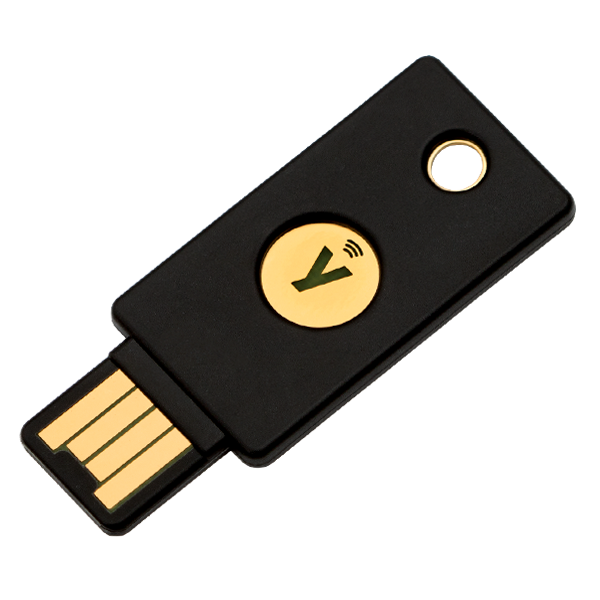
\includegraphics[height=\linewidth]{ubikey}
        \caption{YubiKey\endnote{\url{https://media.yubico.com/media/catalog/product/5/n/5nfc_hero_2021.png}}}
      \end{figure}
    \end{column}
  \end{columns}

  \note{
    \begin{itemize}
      \item wurde als sehr sichere, und trotzdem nutzerfreundliche Methode konzipiert
            \begin{itemize}
              \item[\textrightarrow] deshalb besonders interessant, wie Nutzer dies empfinden
            \end{itemize}
      \item Sicherheitsrisiko: Verlieren des Tokens
            \begin{itemize}
              \item[\textrightarrow] besteht allerdings auch bei anderen Methoden
            \end{itemize}
    \end{itemize}
  }
\end{frame}
